\section{Virzītais nozarotājs}
Virziena jaudas nozarotājs ir četru portu sistēma, kur viens ports ir izolēts no ieejas porta. Visi četri porti ideālā gadījumā ir salāgoti, un shēma ideālā gadījumā ir bez zudumiem. Nozarotāju var realizēt nesimetriskās un simetriskās mikroslokšņu līnijās, koaksiālajos kabeļos vai viļņvados. Tos visbiežāk izmanto signālu caurejošā signāla nolasei kā izstarotā un atstarotā jauda. Nozarotājā optimālā elektromagnētiskā saite starp līnijām tiek sasniegta, ja līniju sasaistītā posma garums ir vesels skaits ceturtdaļvilņu. Nozarotājs darbojās uz elektromagnētiskā principa, caurplūstošā strāva veido elektromagnētisko lauku, kas inducē strāvu izolētajā daļā, pārnesot signālu no viena atzara uz otru. Zemāk redzamais virziena atzarotājs ir izstrādāts X-joslas pastiprinātāja blokā, kur tiek piemeklēts risinājums vidējās jaudas mērīšanai.
\begin{figure}[H]
	\centering
    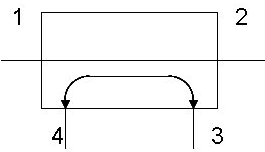
\includegraphics[width=0.9\textwidth]{pictures/bi-directional_coupler.png}\hspace{1cm}
    \caption{Atzarotāja elektriski principiālais apzīmējums}
\end{figure}
